%\documentclass[review]{elsarticle}
%\documentclass[5p]{elsarticle}
\documentclass[utf8]{frontiersSCNS}
%\documentclass{frontiersSCNS}

\usepackage{url,hyperref,lineno,microtype,subcaption}
\usepackage[onehalfspacing]{setspace}

\linenumbers

%\usepackage{lineno,hyperref}
\usepackage[separate-uncertainty=true,multi-part-units=single,range-phrase=--]{siunitx}
\usepackage{color}
%\modulolinenumbers[5]
\usepackage{mhchem}
%\usepackage{enumitem}
%\usepackage{amsmath}
\usepackage{trackchanges}
\usepackage{ulem}
%\usepackage{enumerate}
\graphicspath{{Figures/}}

%\journal{Geomorphology}



\newcommand{\COMON}{\begin{color}{blue}}
\newcommand{\COMOFF}{\end{color}}

\newcommand{\alon}{\begin{color}{red}}
\newcommand{\aloff}{\end{color}}

\newcommand{\GSon}{\begin{color}{orange}}
\newcommand{\GSoff}{\end{color}}

\newcommand{\CPon}{\begin{color}{green}}
\newcommand{\CPoff}{\end{color}}



%% APA style
%\bibliographystyle{model5-names}\biboptions{authoryear}

%\addeditor{Alain}

%%%%%%%
% The trackchanges package adds five new LaTeX commands:
%
%  \note[editor]{The note}
%  \annote[editor]{Text to annotate}{The note}
%  \add[editor]{Text to add}
%  \remove[editor]{Text to remove}
%  \change[editor]{Text to remove}{Text to add}
%
% complete documentation is here: http://trackchanges.sourceforge.net/
%%%%%%%


\def\keyFont{\fontsize{8}{11}\helveticabold }
\def\firstAuthorLast{Pacheco {et~al.}} %use et al only if is more than 1 author
\def\Authors{Marcus Pacheco\,$^{1,*}$, Alain Plattner\,$^{2}$, Greg Stock\,$^{3}$ and Christopher Pluhar\,$^{1}$}
% Affiliations should be keyed to the author's name with superscript numbers and be listed as follows: Laboratory, Institute, Department, Organization, City, State abbreviation (USA, Canada, Australia), and Country (without detailed address information such as city zip codes or street names).
% If one of the authors has a change of address, list the new address below the correspondence details using a superscript symbol and use the same symbol to indicate the author in the author list.
\def\Address{$^{1}$Earth \& Environmental Sciences, California State University, Fresno, Fresno, CA, USA \\
  $^{2}$ Geological Sciences, University of Alabama, Tuscaloosa, AL, USA\\
  $^{3}$ National Park Service, Yosemite National Park, CA, USA }
% The Corresponding Author should be marked with an asterisk
% Provide the exact contact address (this time including street name and city zip code) and email of the corresponding author
\def\corrAuthor{Marcus exact address}

\def\corrEmail{Marcus email, or should we put alain email, in case MArcus' fresno state email disappears?}






\begin{document}

\onecolumn
\firstpage{1}

%\begin{frontmatter}

\title[Royal Arches Meadow rock avalanche]{Three-dimensional Geophysical Imaging of the Royal Arches Meadow Rock Avalanche in Yosemite Valley, California}

\author[\firstAuthorLast ]{\Authors} %This field will be automatically populated
\address{} %This field will be automatically populated
\correspondance{} %This field will be automatically populated

\extraAuth{}% If there are more than 1 corresponding author, comment this line and uncomment the next one.
%\extraAuth{corresponding Author2 \\ Laboratory X2, Institute X2, Department X2, Organization X2, Street X2, City X2 , State XX2 (only USA, Canada and Australia), Zip Code2, X2 Country X2, email2@uni2.edu}


%% %% Group authors per affiliation:
%% \author[Marcus]{Marcus Pacheco\corref{cor1}}
%% \address[Marcus]{Earth \& Environmental Sciences, California State University, Fresno}
%% \cortext[cor1]{Corresponding author.}
%% \ead{mvpacheco90@mail.fresnostate.edu}

%% \author[Alain]{Alain Plattner}
%% \address[Alain]{Geological Sciences, University of Alabama}

%% \author[Greg]{Greg Stock}
%% \address[Greg]{National Park Service, Yosemite National Park}

%% \author[Chris]{[Christopher Pluhar}
%% \address[Chris]{Earth \& Environmental Sciences, California State University, Fresno}


\maketitle
										\begin{abstract}
\section{}										

Rock avalanches have occurred intermittently in Yosemite Valley, California, since the retreat of glaciers at the end of the last ice age \SI{\approx15}{\kilo a}. The Royal Arches Meadow rock avalanche is an approximately \SI{0.5e6}{m^3} deposit of rock debris located in eastern Yosemite Valley. Cosmogenic beryllium-10 exposure ages of boulders on the deposit indicated that the rock avalanche occurred at \SI{14+-0.3}{\kilo a}, shortly after deglaciation. The interface between the rock avalanche deposit and the underlying fluvial, deltaic, and lacustrine sediments therefore provides a reference for the valley surface at that time. To investigate amd locate this interface, we collected eight Ground Penetrating Radar (GPR) and five Electrical Resistivity Tomography (ERT) profiles longitudinally and transversely crossing the rock avalanche. Both methods are sensitive to the contrast between the granitic avalanche deposit and the underlying sediments. We identified multiple reflectors in the GPR data that are continuous across the profiles, while ERT inversion results along the same profiles showed resistive material (\SIrange{1000}{8000}{\ohm.m}) overlying relatively conductive material (\SI{<1000}{\ohm.m}). By constraining ERT inversions with picked GPR reflectors, we identified a single GPR reflector that separates resistive material on top from relatively conductive material underneath. This reflector is approximately horizontal at an average elevation of ~1207 m. We interpret this interface as the bottom of the rock avalanche and hence as the surface of Yosemite Valley at the end of the last glaciation. Thus, we estimate that \SI{10}{m} of total aggradation have occurred on the terrace adjacent to the rock avalanche since emplacement. Our findings collaborate with the reconstruction of the sedimentation history and landscape evolution of Yosemite Valley. Moreover, the identification of bottom of the RAMRA using geophysical methods, provided us insights into how to imrpove volume estimation for similar deposits.     
y.

\tiny
\keyFont{\section{Keywords:}Rock Avalanche, Ground Penetrating Radar, Electrical Resistivity Tomography, Yosemite Valley, Near-surface Geophysics}
%All article types: you may provide up to 8 keywords; at least 5 are mandatory.
                                                                                \end{abstract}

%\begin{keyword}
%GPR \sep ERT \sep Yosemite
%\texttt{elsarticle.cls}\sep \LaTeX\sep Elsevier \sep template
%\MSC[2010] 00-01\sep  99-00
%\end{keyword}

	                                                                        %\end{frontmatter}

%\linenumbers






\section{Introduction}

Large rock slope failures such as rock avalanches are among the most efficient processes changing mountainous landscapes \COMON (REFERENCES HERE) \COMOFF. In Yosemite Valley, California, rock slope failures not only poses a serious hazard to the nearly four million yearly visitors, but also to the park infrastructure. In this project, we explore (describe?) how we used one of those large rock slope failure deposit in the valley, to gain insights into the local sedimentation history and landscape evolution. 

Unlike Rockfall, which happen very frequently in the park and produce small volume of debris, rock avalanches are rare, and typically move large masses of material over long distances in a matter of seconds (Stock and Uhrhammer, 2010). Consequently, these events are an important geomorphic process reshaping the landscape of Yosemite Valley. Postglacial massive rock debris deposits, such as rock avalanches,  are well preserved in Yosemite Valley \COMON (REFERENCE HERE) \COMOFF, and can provide us with a position marker of the valley floor during the time that they occurred


\subsection{Physical Setting}

Yosemite Valley was initially carved by fluvial incision, and latter deepened by several glaciation cycles over the past few millions of years. The most recent glaciation is locally known as Tioga glaciation. It peaked between \num{28000} and \num{17000} years BP and only partially filled  Yosemite Valley (\cite{huber1987geologic}). Subsequently, the Valley is thought to have been deglaciated somewhen between \num{15000} and \num{17000} years ago (\cite{huber1987geologic};  \cite{Wieczorek+1996}.

Unlike other U-shaped glacial valleys, Yosemite valley has an U-shape with a long and flat topography. The present flat and broad flood plain of Yosemite Valley is meandered by the Merced River and Tenaya creek \cite{Wieczorek+1996}. Flanked by up to \SI{1000}{m} tall and steep granitic rock faces (\COMON Stock and Uhrhammer, 2010 \COMOFF). The main reason for the flat valley surface is the deposition of glacial, lacustrine, deltaic and fluvial sediments during deglaciation periods \COMON reference \COMOFF. The valley fill has a depth of up to \SI{600}{m} \cite{gutenberg1956seismic},


    
\subsection{Slope Failures In Yosemite Valley}

Because of  the nearly vertical and sometimes overhanging walls, slope failures events such as rock falls, rock slides, and debris flows are common in Yosemite Valley. Most of those deposits are concentrated relatively close to the cliffs where they originated. However, at ten locations in Yosemite Valley , rock debris have traveled hundreds of meters onto the valley \COMON(REFERENCE HERE)\COMOFF. Those deposits were termed Rock Avalanches, because of their distinct hummocky morphology, run out of hundreds of meters, and volumes in the hundreds of thousands of m3 \COMON(Stock 2014, Evans 2006,  Hungr 2014, Wieczorek 1998, Stock 2010, Stock 2011)\COMOFF. 


\subsection{Royal Arches Meadow Rock Avalanche}\label{sec:introRAMRA}

The Royal Arches Meadow Rock Avalanche (RAMRA) lies in the eastern Yosemite Valley, inside Yosemite National Park in California, USA (Fig.~\ref{Study_Area}. Talus deposits cover the RAMRA at Northeast, and at Southwest of the avalanche, lies a fluvial terrace, as well as the Tenaya creek cut bank and active channel (Fig.~\ref{RAMRA} A). 


\begin{figure*}[h]
  
  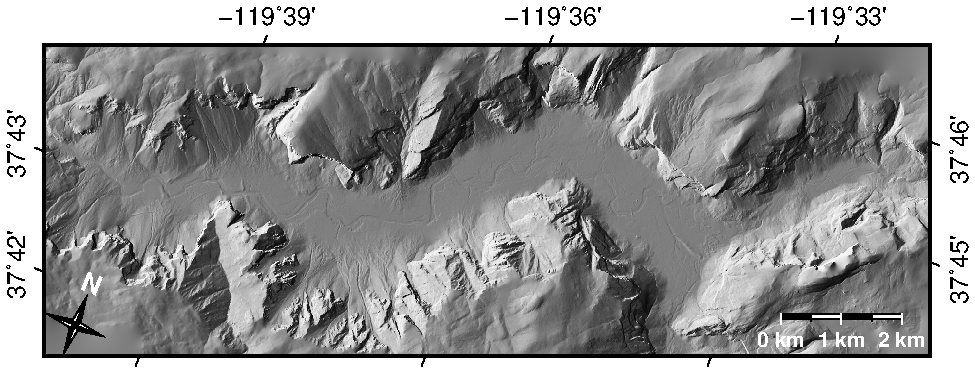
\includegraphics[width=\textwidth]{Yosemite.pdf}
  \caption{Yosemite Valley Map View, white star highlight the study area.  \label{Study_Area}}
        
\end{figure*}


The highlighted portion marked in the map as RAMRA (Fig.~\ref{RAMRA} A), is actually the distal portion of the surface expression of the Royal Arches Meadow Rock Avalanche. Contrasting with the steep angle (~XX) of adjacent talus deposits, the avalanche presents an overall shallow angle of ~YY \COMON Greg, do you know these angles? \COMOFF, and a hummocky morphology. The avalanche is also marked by boulders ranging from tens of centimeters to several meters tall (Fig.~\ref{RAMRA} B and C).

The presence of boulders completely disappear Southwest of the rock avalanche area, and the topography become flat until the edge of the Tenaya creek cut bank, where the elevation drops in about 5 m. 



\begin{figure*}[h]
  
  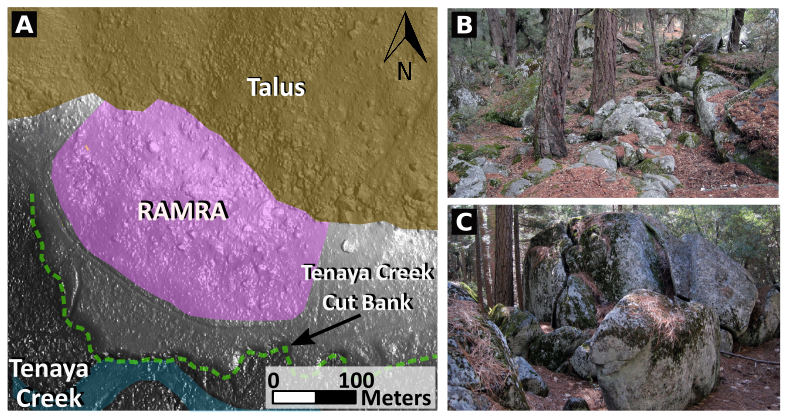
\includegraphics[width=\textwidth]{RAMRA.png}
  \caption{(A) Map view of the study area highlighting the local geomorphology, (B) and (C) are pictures of the surface morphology of the RAMRA.  
    \label{RAMRA}}
  
\end{figure*}



Cosmogenic \ce{^{10}Be} exposure ages demonstrate that the Royal Arches Meadow Rock Avalanche happened \SI{14030 +- 340}{a}. This makes the RAMRA the oldest avalanche in the park. More importantly, because this event happened shortly after the Last Glacial Maximum in the valley (\SI{15000}{a}), the interface between the bottom of the RAMRA and the underlying paleo-valley marks the position of the valley shortly after the LGM. This boundary represent an important marker to understand the sedimentological and landscape evolution of the Yosemite Valley, and therefore it is our target of study. Because this interface is not exposed in the surface, we combined geophysical methods to locate the position of the bottom of the RAMRA in subsurface, and used Cosmogenic beryllium-10 ages to estimate the age of the avalanche, and therefore  gain insights into the rates of local deposition.

% Hi Greg, I was previously using the age of the RAMRA to link it with the LGM, and to provide some closure to the intro by stating our goals. However, now that we are including the ages in the paper, I wonder if there is a better way to phrase it here without being repetitive, but at the same time keeping the essential idea.


%\bigskip

                 
                 
\subsection{Geophysics and Slope Failures Deposit}s

\alon\sout{To obtain spatially continuous information of the bottom of
  the RAMRA,} [@Marcus: The paper is all about studying the bottom of
  the RAMRA, so you can directly go to ``how''] \aloff We used a
combination of two non-intrusive geophysical methods --- Electrical
Resistivity Tomography (ERT) and Ground Penetrating Radar
(GPR). Geophysical methods have been successfully applied to image
slope failures deposits (e.g., \cite{sass2006determination};
\cite{otto2006comparing}; \cite{socco2010geophysical};
\cite{brody2015near},\cite{liu2018near}) \alon [This sequence of
  sentences in this paragraph is odd. You probably want to start with
  explaining the two methods you use (the next paragraph). Then talk about
  the different studies you cite and what methods they use in which
  combination and what context. Why do you use the ones you use (GPR and ERT), how is this in
  context to what other people used? Are you one of the few using
  these methods, or are these the two standard methods? Then put in a
  connecting sentence to the next paragraph, such as ``For our
  purposes, GPR and ERT are ideally suited as we lay out in the
  following''] \aloff.
                 
Ground Penetrating Radar is a geophysical technique that detects electrical discontinuities in the shallow subsurface (typically < 50 m) using the emission of electromagnetic waves \citep{neal2004ground}. The most common form of GPR measurements, called common offset profiling, involves keeping a transmitter antenna and a receiver antenna at a fixed distance and moving them along a profile line on the surface to detect reflections from subsurface features \citep{jol2008ground}. GPR reflections are caused by abrupt changes in dielectric permittivity of the medium. Several factors can influence those changes, such as: different lithologies, variations in grain size and orientation, and water table (Olhoeft, G. R., 1998 and \citep{neal2004ground}. Hence, GPR is an adequate technique to investigate the interface between the  granitic debri avalanche deposit and the underlying  valley sediments (lascustrine, deltaic and fluvial).   

On the other hand, Electrical Resistivity Tomography operates by measuring voltage differences caused by electric currents that are injected into the ground. Overlapping measurements can then, with the help of computational inversions, be turned into images of the electrical resistivity variation within the subsurface. These procedures are typically underdetermined, presenting multiple possible solutions. We hence can greatly improve the reliability of our solutions by providing additional constraints in the form for example of known interfaces (Oldenburg 1999; Loke 2013). ERT is an efficient technique to image contrasts in electro resistivity. In our study area, the electro resistivity contrast is caused mostly by the distinct  lithology, grain size, sorting, porosity, and water content  of rock avalanche that covers much finner valley sediments. 


Geophysical methods present a efficient way to acquire subsurface information and  to cover large areas where direct physical contact (e.g., sampling, coring) is difficult or not possible. However, geophysical methods always contain a degree of  uncertainty and ambiguity. In order to minimize those effects and therefore to ensure that the images created by the geophysical data emulate well the real geological setting, it is important to not only compare different geophysical methods, but also to combine them. \COMON Doetsch, Linde, Pessognelli, Green, \& G\"unther, (2012)\COMOFF, have demonstrated the effectiveness of using Ground Penetrating Radar reflectors to constrain electrical resistivity tomography (ERT). This technique operates by offering the option of removing smoothness across the interfaces identified in the GPR data in the ERT inversion 

\COMON Hi Alain, would you have more examples to go here? I have browsed the internet, but were not able to find any major paper about this combination. 

Giving the public who will read the paper, I was also wondering if
we should write 2 or 3 sentences clarifying (in very simple words)
the  non-unique cachracter of ERT inversions.\COMOFF.

\alon
@Marcus: Yes, explain the non-unique character of ERT. This is key to
why we even need GPR and what you are doing in the following. For the
examples: I would recommend looking through Doetsch's paper and seeing
who they cite. Then cite these people and continue the lit-research by
following to who they cite, etc. 
\aloff



%\bigskip   



\section{Methods}

\subsection{Geophysics}

We collected eight Ground Penetrating Radar
    (GPR) and five Electrical Resistivity Tomography (ERT) profiles
    longitudinally and transversely crossing the rock avalanche
    (Fig.~\ref{GPR_ERT_Map} A and B), covering both exposed parts of the rock
    avalanche, and the adjacent area.\alon Marcus, I'm assuming that
    you mean GPR ERT Map (not GPR ERT MapT) for the figure you
    reference. Is that right? \aloff

For the GPR profiles, we used a Sensors \& Software PulseEKKO Pro (\SI{50}{\mega Hz}) system to acquire data during the months of September and October of 2018. We processed these profiles using GPRPy \citep{plattner2019comunity,Plattner2019}, applying a time zero correction, filter (dewow and mean trace removal), T-power gain, f-k migration \citep{stolt1978migration} and topographic correction. We used 0.11 m/ns wave velocity, which we obtained from a Wide Angle Reflection and Refraction survey (WARR) on site. Raw data and GPRPy processing scripts are included in the supplemental material of this article. We then used the processed profiles to track the lateral continuity of specific reflectors between the profiles following the methodology proposed by \citep{mitchum1977seismic}.

We also collected Five ERT transects at the study area, using the Advanced Geosciences Inc SuperSting R1 (28 electrodes), with an electrode spacing of six meters, and a Wenner–Schlumberger and dipole-dipole acquisition scheme. Subsequently, the ERT data were filtered using DC2DInvRes \COMON (REFERENCE) \COMOFF and inverted using BERT/GIMLi (\cite{gunther2006three} and (\cite{Ruecker2017}).


								 \begin{figure*}[h]

	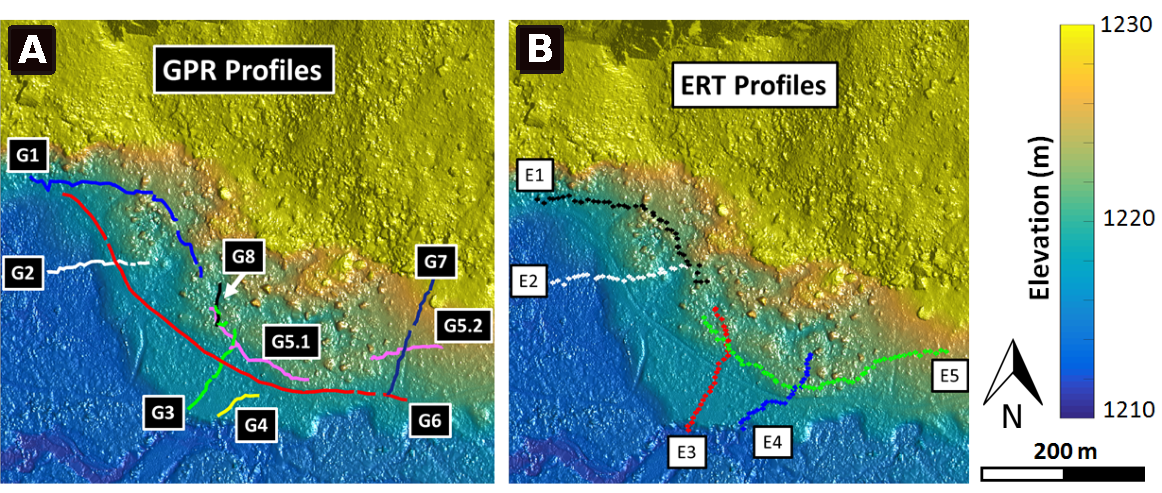
\includegraphics[width=\textwidth]{Figures/GPR_ERT_Map.pdf}
		\caption{:(A) Map view of GPR profiles, and (B) map view of ERT profiles. \label{GPR_ERT_Map}}

								   \end{figure*}



\subsection{RAMRA Age}

-Cosmogenic be 10 in 3 locations

-Cosmogenic beryllium-10 ages yield a mean exposure age of 15.3 +- 1.4 ka


%\bigskip  

 
\section{Results}


\subsection{GPR Results}

\alon Here you need to include the velocity analysis. Perhaps also put
its coordinates on the map.\aloff


\COMON Hi Alain, I am afraid that if we include the position of the WARR on the map it is going to get even more polluted.
        additional. giving the public for this paper, do you believe worth it to explain the velocity analysis process? In methods I briefily mentioned that we did a WARR and used 0.11 as velocity. We can also include some citations for the WARR \COMOFF


We observed the following patterns of reflection in the GPR profiles (Fig.~\ref{GPR_Oblique}A): (A) A strong plan-parallel reflector (Alpha) is visible in all GPR profiles varying from 1216 until 1214 m of elevation. (B) Bellow 1214-1212 m of elevation, the pattern of reflectors change to a chaotic geometry as the radar signal gets scattered, this pattern is limited at bottom  by a nearly horizontal reflector (Beta)  at the elevation of ~1207 m. Lastly, in profiles G2,  G3, G4, G5, G6, and G7 another strong continuous reflector is identified at the elevation of ~1205m (Gamma) (Fig.~\ref{GPR_Oblique}B). 

The reflectors named Alpha, Beta and Gamma were observed in several of the collected profiles, and appear at a consistent elevation \COMON (Table 1) \COMOFF, varying no more than 1.5 m downslope (Fig.~\ref{GPR_Oblique}B). lastly, we interpolated the elevation information extracted from those reflectors to emulate the lateral continuity of those interface in three dimensions (Fig.~\ref{GPR_Oblique}C).  


								 \begin{figure*}[h]

	\includegraphics[width=\textwidth]{Figures/GPR_Oblique.pdf}
		\caption{:(A) Oblique view of GPR profiles looking towards NW, (B) Tracked Reflectors Alpha, Beta, and Gamma, and (C) Interpolated surface for reflector Beta. \label{GPR_Oblique}}

								   \end{figure*}
								   
\begin{itemize}
    \item Table 1 here
\end{itemize}			   

								   
\subsection{Constraining ERT Results with GPR Reflectors}

We observed relative resistive material (1k-8k ohm m) overlying relatively conductive material (<1k ohm m) for all ERT inverted profiles (Fig.~\ref{ERT_inversion}A). Moreover, the ERT inversion using the elevation information from GPR reflectors demonstrated that Reflector Beta best constrained the inversion, by creating a sharp interface between resistive/conductive material (Fig.~\ref{ERT_inversion}C).. This result is consistent for ERT profile E1, E2, E3, and E5. 

							 \begin{figure*}[h]

	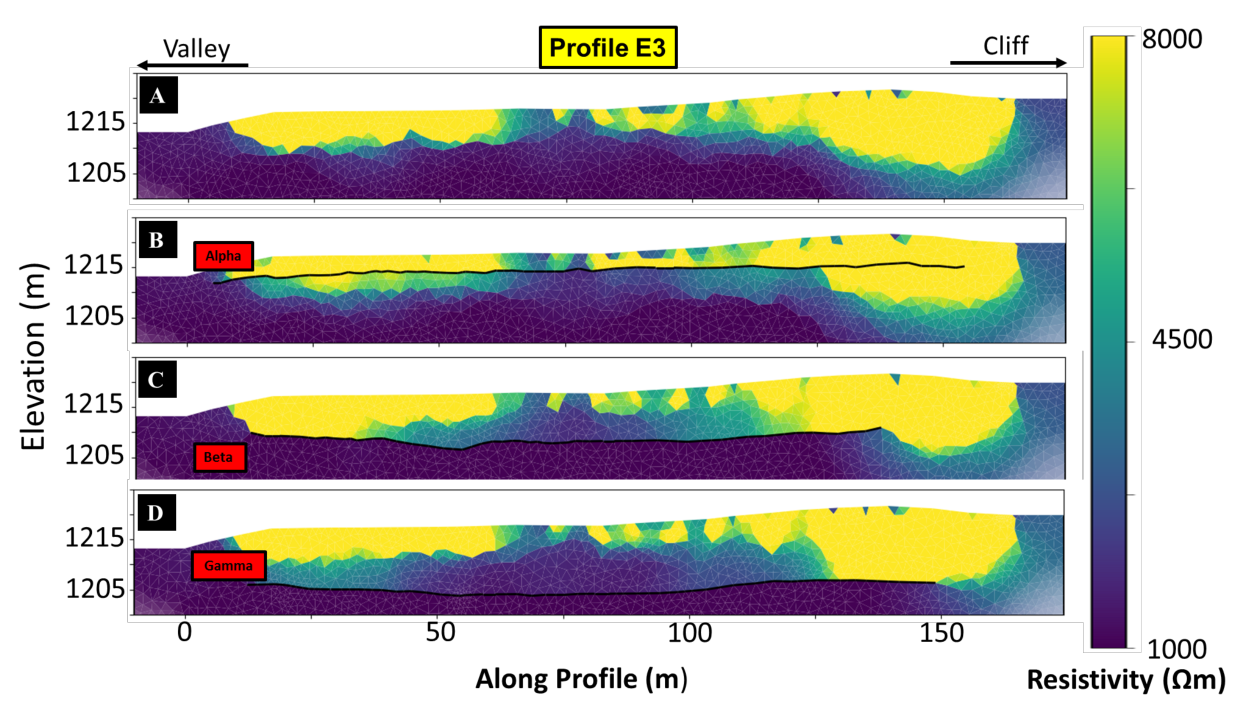
\includegraphics[width=\textwidth]{Figures/ERT_inversion.pdf}
		\caption{Inverted results for profile E3: (A) ERT inversion, (B) ERT inversion using reflector Alpha, (C) ERT inversion using reflector Beta, and (D) ERT inversion using reflector Gamma.\label{ERT_inversion}}

								   \end{figure*}

%\bigskip


\section{Discussion}

Based on the observation obtained from of the geophysical data, we interpreted Beta reflector as the interface between the Royal Arches Meadow Rock Avalanche and the underlying paleo-valey floor (Fig.~\ref{GPR_Oblique} B). The following reasons support this idea: 

\begin{enumerate}[I]
\item Reflector Beta present a strong reflection, most likely becayse of the contrasting dielectric properties from the rock avalanche and underlying palleo-valley floor sediments. 
\item Reflector Beta presents lateral continuity equivalent to the range of the rock avalanche observed in the surface.  
\item The presence of resistive material overlying relatively conductive material in an approximately elevation of 1207 m (Beta average elevation ). 
\item Beta is the GPR reflector that best remove the smoothness during the ERT inversions, creating a sharp transition between resistive and non-resistive material.
\item  \COMON Reflector configuration? \COMOFF 
\end{enumerate}



\subsection{Covering Gaps in the Geophysical Data}

Because of the difficulties imposed by the field of study (e.g. big boulders,  large fallen trunks) and the broad area covered by the avalanche, we were not able to collect a dense grid of geophysical data on the top of the rock avalanche. Applying two different geophysical methods was helpful, since we were able to collect ERT data where the logistics for GPR would not work, and vice versa. 

To overcome the lack of data from one of the methods in specific locations, we made two simple assumptions to interpret the data based in the overall pattern observed: (I) the rock avalanche overlay the valley sediments and it is more resistive; (II) the position of reflector Beta is consistent at an average elevation of 1207 m.  

For example, in profile G5.1, we observed a strong signal attenuation below the elevation of 1212 m (Fig.~\ref{Combined_ABCD}A), making it really difficult to identify the position of reflector Beta. But because the nearby profiles show reflector Beta at elevation of 1207 m, we can make the educated guess of placing/tracking a relatively flat reflector at elevation of 1207 in this profile (Fig.~\ref{Combined_ABCD}B). Subsequently, we run the ERT inversion including the inferred profile (1207 m) as well as the other observed profiles (Fig.~\ref{Combined_ABCD}B). Then, we observed that the inferred Beta profile at elevation of 1207 m, is the one that best constrains the data creating the expected contrast in resistivity (Fig.~\ref{Combined_ABCD}D).  


				(Fig.~\ref{Combined_ABCD})			

                                \begin{figure*}[h]

	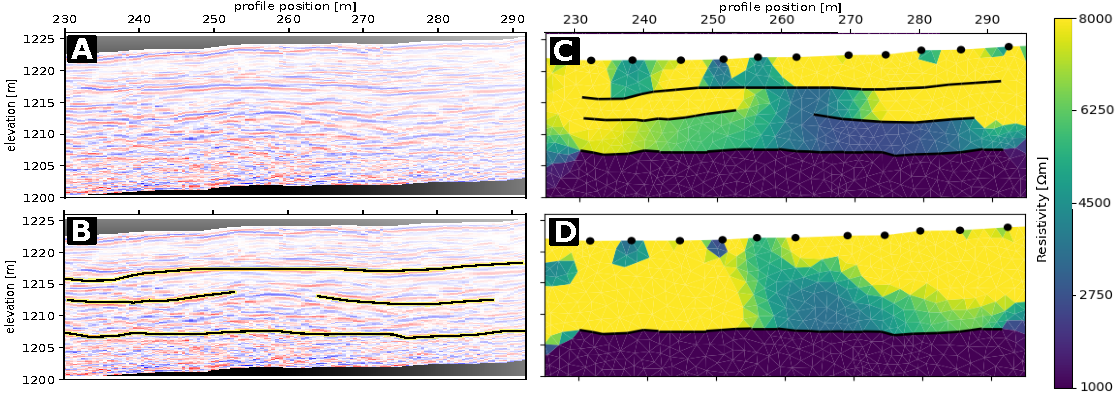
\includegraphics[width=\textwidth]{Figures/Combined_ABCD.pdf}
		\caption{:(A) Oblique view of GPR profiles looking towards NW, (B) Tracked Reflectors Alpha, Beta, and Gamma, and (C) Interpolated surface for reflector Beta. \label{Combined_ABCD}}

								   \end{figure*}



\subsection{Resistive Material Beyond the RAMRA Area}

\COMON Hi everybody, do you believe worth it to speculate/talk why there are resistive material beyond where we can see the rock avalanche in the surface \COMOFF

Resistive material appears overlaying relatively conductive material
beyond the area mapped as the exposed portion of the rock avalanche
(beginning of profiles E2, E3, and E4
(Fig.~\ref{GPR_ERT_Map}B)). \alon Marcus, I assume that here you mean
GPR ERT Map (not GPR ERT MapT) for the figure reference. Right? \aloff 

Although this area presents the pattern of resistive material overlaying relatively conductive material, it is unlikely that this resistive material is the continuation of the rock avalanche. Several evidences points to this conclusion: The area does not present boulders in the surface, nor a hummocky morphology. Additionally, the exposed cut bank of the Tenaya creek (Fig.~\ref{RAMRA} A), and where profiles E3 and E4 starts, and half-way through profile E2 shows fluvial deposits, and no sign of an rock avalanche deposit.  


\subsection{Aggradation Rate since the LGM}

Because of the age of the Royal Arches Meadow Rock avalanche deposit, it is possible to use the bottom of the avalanche (~1207 m) as a marker of the position of the valley shortly after the Last Glacial Maximum in the valley. This then can give us insights into the rates of aggradation since the LGM. 

For example, the fluvial terrace of the Tenaya creek, located ~ 200 m southwest of the distal portion of the rock avalanche has a present elevation of ~1217 m., and if the position of the valley floor during the LGM is ~1207, we can infer that at least 10 m of local aggradation has occurred. 


\subsection{Volume}

\COMON Hi Greg, could you please elaborate here or in a previous section how you estimated the Volume for the RAMRA (surface and subsurface).
\COMOFF

-Distal volume estimation considering the bottom of the rock avalanche as the present valley floor =  378,000 m3

-Distal volume estimation considering the bottom of the rock avalanche as the interpreted bottom of the rock avalanche from the geophysical data = 955,000 m3 

-This is not the total volume of the avalanche, but it demonstrate how estimations based on purely surface interpretation can be misleading. Mainly in environments dominated by aggradation. 


%\bigskip  


\section{Conclusions}


As expected the ERT data showed a pattern of resistive material (rock avalanche debris) overlaying relatively conductive material (fluvial, deltaic, and lacustrine sediments). However, it was only with a combination of GPR and ERT that we were able to estimate the elevation (position?) of such contact. And therefore, demonstrating that those two geophysical methods combined are a powerful tool to image bottom of rock avalanches.  

We were able to demonstrate that investigating the subsurface of RAMRA significantly improve volume estimation, and thus hazard assessment 
     
     \COMON 
     This proved true for ONE rock avalanche that we studied, and might not be true for other rock avalanches. I am trying to convert this idea to:
     - Subsurface investigation improved the volume estimation of the RAMRA,
     - for large rock avalanches, the deposit in the subsurface should not be ignored,
     - improving rock avalanche volume estimation collaborates with hazard assement. 
      \COMOFF. 



\section*{Conflict of Interest Statement}
%All financial, commercial or other relationships that might be perceived by the academic community as representing a potential conflict of interest must be disclosed. If no such relationship exists, authors will be asked to confirm the following statement: 

The authors declare that the research was conducted in the absence of any commercial or financial relationships that could be construed as a potential conflict of interest.


\section*{Author Contributions}

The Author Contributions section is mandatory for all articles, including articles by sole authors. If an appropriate statement is not provided on submission, a standard one will be inserted during the production process. The Author Contributions statement must describe the contributions of individual authors referred to by their initials and, in doing so, all authors agree to be accountable for the content of the work. Please see  \href{http://home.frontiersin.org/about/author-guidelines#AuthorandContributors}{here} for full authorship criteria.


\section*{Funding}
Details of all funding sources should be provided, including grant numbers if applicable. Please ensure to add all necessary funding information, as after publication this is no longer possible.


\section*{Acknowledgments}
This is a short text to acknowledge the contributions of specific colleagues, institutions, or agencies that aided the efforts of the authors.

\section*{Supplemental Data}
 \href{http://home.frontiersin.org/about/author-guidelines#SupplementaryMaterial}{Supplementary Material} should be uploaded separately on submission, if there are Supplementary Figures, please include the caption in the same file as the figure. LaTeX Supplementary Material templates can be found in the Frontiers LaTeX folder.

\section*{Data Availability Statement}
The datasets [GENERATED/ANALYZED] for this study can be found in the [NAME OF REPOSITORY] [LINK].
% Please see the availability of data guidelines for more information, at https://www.frontiersin.org/about/author-guidelines#AvailabilityofData



\bibliographystyle{frontiersinSCNS_ENG_HUMS}
\bibliography{mybibfile}

\end{document}
